%%% LaTeX Template: Article/Thesis/etc. with colored headings and special fonts
%%%
%%% Source: http://www.howtotex.com/
%%% Feel free to distribute this template, but please keep to referal to http://www.howtotex.com/ here.
%%% February 2011
%%%
%%% Last updated September 2018 by CDM

%%%  Preamble
\documentclass[11pt,letterpaper]{article}
\usepackage[margin=1.0in]{geometry}
\usepackage[T1]{fontenc}
\usepackage[bitstream-charter]{mathdesign}
\usepackage[latin1]{inputenc}					
\usepackage{amsmath}						
\usepackage{xcolor}
\usepackage{cite}
\usepackage{hyphenat}
\usepackage{graphicx}
\usepackage{float}
\usepackage{subfigure}
\usepackage{sectsty}
\usepackage[compact]{titlesec} 
\usepackage[tablegrid]{vhistory}
\allsectionsfont{\color{accentcolor}\scshape\selectfont}

%%% Definitions
\definecolor{accentcolor}{rgb}{0.0,0.0,0.5} 
\newcommand{\teamname}{Code Blink}
\newcommand{\productname}{Smart Shutter}
\newcommand{\coursename}{CSE 4316: Senior Design I}
\newcommand{\semester}{Fall 2019}
\newcommand{\docname}{Project Charter}
\newcommand{\department}{Department of Computer Science \& Engineering}
\newcommand{\university}{The University of Texas at Arlington}
\newcommand{\authors}{Alejandro Escobar\\ Umesh Shrestha\\ Khoa Huynh\\ Tamunonengiye Nga \\ Jose Quintero}

%%% Headers and footers
\usepackage{fancyhdr}
	\pagestyle{fancy}						% Enabling the custom headers/footers
\usepackage{lastpage}	
	% Header (empty)
	\lhead{}
	\chead{}
	\rhead{}
	% Footer
	\lfoot{\footnotesize \teamname \ - \semester}
	\cfoot{}
	\rfoot{\footnotesize page \thepage\ of \pageref{LastPage}}	% "Page 1 of 2"
	\renewcommand{\headrulewidth}{0.0pt}
	\renewcommand{\footrulewidth}{0.4pt}

%%% Change the abstract environment
\usepackage[runin]{abstract}			% runin option for a run-in title
%\setlength\absleftindent{30pt}			% left margin
%\setlength\absrightindent{30pt}		% right margin
\abslabeldelim{\quad}	
\setlength{\abstitleskip}{-10pt}
\renewcommand{\abstractname}{}
\renewcommand{\abstracttextfont}{\color{accentcolor} \small \slshape}	% slanted text

%%% Start of the document
\begin{document}

%%% Cover sheet
{\centering \huge \color{accentcolor} \sc \textbf{\department \\ \university} \par}
\vspace{1 in}
{\centering \huge \color{accentcolor} \sc \textbf{\docname \\ \coursename \\ \semester} \par}
\vspace{0.5 in}
\begin{figure}[h!]
	\centering
   	
\includegraphics[width=0.40\textwidth]{images/smart_shutter}
\end{figure}
\vspace{0.5 in}
{\centering \huge \color{accentcolor} \sc \textbf{\teamname \\ \productname} \par}
\vspace{0.5 in}
{\centering \large \sc \textbf{\authors} \par}
\newpage


%\vspace{1 in}
%\centerline{January 13th, 2012}
%\newpage

%%% Revision History
\begin{versionhistory}
  	\vhEntry{0.1}{09.13.2019}{KH}{document creation}
  	\vhEntry{0.2}{09.23.2019}{KH|AE|US}{complete draft}
  	\vhEntry{0.3}{09.30.2019}{KH|US|TN|JQ|AE}{release candidate 1}
  	\vhEntry{1.0}{10.01.2019}{KH|TN|US|JQ|AE}{official release}
  
\end{versionhistory}
\newpage

%%% Table of contents
\tableofcontents
\newpage

%%% List of figures and tables (optional)
\listoffigures
%\listoftables
\newpage
\setcounter{table}{0}

%%% Agile project charter sections
\section{Vision}
Wouldn't it be great if you could control the amount of natural light entering your house or complex at the touch of a button on your smartphone? Now, a person will be able to control one specific sun blind in a room, or even all the sun blinds in an entire complex in no time, with little to no effort. This is great for those who have physical difficulties, or simply those who aspire to have a fully automated home.
\section{Mission}
Smart Shutter is a project in which our team along with EE and embedded development teams are creating the standard shutter can be controlled by a mobile app. The app will work on android phone or an iPhone and it will help to move and position the louvers  in required angle by a user. These shutters are produced to be used in commercial building like hospital , business area or retirement homes. The blinds can be used in small scale too.\newline
Since 3 teams are working collaboratively in this project, EE teams will develop motor controller and control board. Embedded development team and our teams will work in microcontroller firmware, communication protocol and app interface. The first and foremost mission in this project is to meet with all the teams and sponsors and decide what should be done by each team. Since our application team is to develop the app that can connect with the shutter controller device through Wi-Fi or Bluetooth and able to control the shutter through the app. The mission of our team is that the app is simpler and easy to use. We are  trying to make the app where we can scan the shutter via barcode and schedule the time at certain angle at given time and date. 

\section{Success Criteria}
Upon completion of this prototype application, we expect the following success indicators to be observed on the Smart Shutters implementing our application software. \newline
\begin{itemize}
\item The application will accomplish a full functioning interface without bugs
\item The application will establish a connection to multiple Smart Shutters
\item The application will have a functioning preset timer that adjusts the corresponding shutters at the scheduled time even when the app is closed.
\item The Smart Shutters will finish adjusting within 3 seconds of the action event (pressing an adjustment button) on the application
\end{itemize}
\newpage

%%% Remaining project charter sections
\section{Background}
This project is intended to be deployed to senior citizen homes as well as locations that desire a fully automated louvre control.
Plantation shutters are attractive attachments to any home or building and helps conserve heat as well as requires less intensive cleaning. Because of its benefits, many buildings take to having multiple plantation shutters located in various rooms in various sizes. In some installed spots, it is difficult to reach the shutters and as such are left inaccessible and unused.
 Even though they are great additions to certain homes and buildings, if they are not easy to access, the plantation shutters can be seen as an inconvenience. For easy deployment to retirement homes, it is necessary to simplify the use of these shutters as residents are most likely not in the best physical state to manually handle these shutters.
 The same consideration goes to businesses like hospitals that have large scale shutters located around the premises even within multiple rooms. Having to walk around the halls and operate these shutters probably multiple times a day would be very inefficient and tasking. Using a smartphone application to automatically open and close some or all the shutters in a complex even set controls based on a set schedule would be a massive step in convenience and bringing comfort without added stress
Then of course are the technological-driven individuals who aspire to have fully automated homes. Having a smart shutter that automatically opens and closes the louvres depending on sunrise and sunset as well as a quick option to operate all shutters in a room, a set of rooms or all the rooms with just a click of a button or an easily controlled slider bar would be a huge benefit to them as well as the added edge to their modernized complex.
Thus, the idea to automate plantation shutters came about to promote ease of use and comfort you don't have to work for.

\section{Related Work}

Automation of the surrounding environment of a modern human being allows increasing his work efficiency and comfort.\cite{Patz2013}. Our product is design to help handicap person who disability to walk or can not walk normally to open and shutdown the window by automation.Beside that, our Smart Shutter will be a helpful product for commercial building to control all the windows individual or grouping windows.Bluetooth has become the standard technology for external interfacing to laptop PCs and mobile devices\cite{Hansen} that is the reason why we chose Bluetooth connection for Smart Shutter. Home Automation System (HAS) using Android for Mobile Phone\cite{Panth2011} and we try to do the same thing by using Bluetooth connection for each individual windows. All windows are connected to wireless device and then connect to mobile device. So our product support and application in both android and iOS.Android is a technology platform with its own ecosystem of tools to support it\cite{Gerber}, and we decide to use Android Studio for our Android app.Basic understanding about iOS App Development\cite{Chang} is helping us with iPhone app. By just install our product, customer can open or shut down window all the way or half way depend on what the prefer. They can schedule open and shutdown windows on sunrise and sunset. With our product, customer can enjoyed a nice scene outside just by one second. Imagine about a patient who just have a surgery can open the window without helping form a nurse or another person. It helps the patient for not waiting for help, and also the nurse to save time and help other patient. If one leaf can giving hope like The Last leaf of O'Henry, our Smart Shutter will bring people more for our customer.




\section{System Overview}
\begin{figure}[h!]
    \centering
    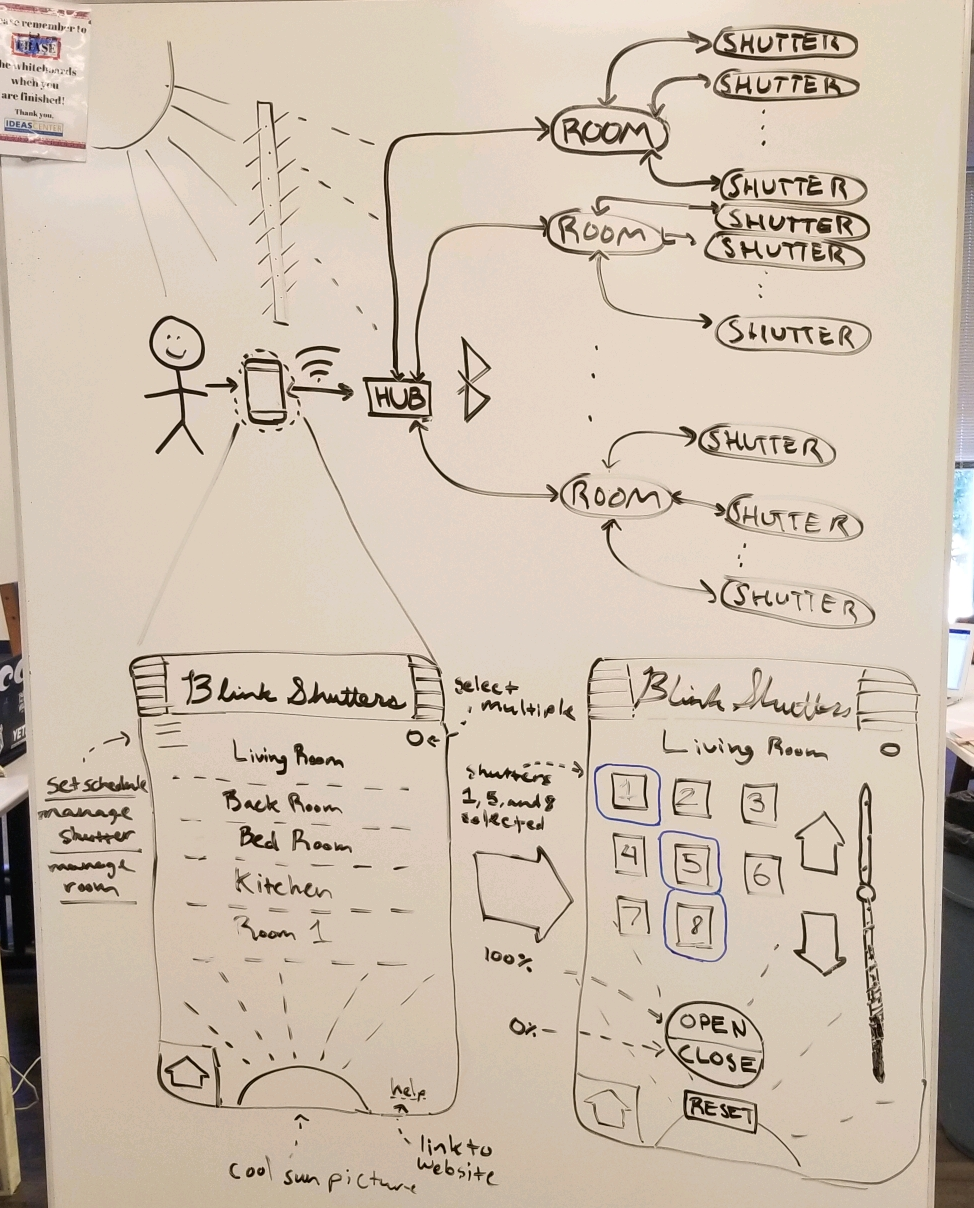
\includegraphics[width=0.5\textwidth]{images/picture}
    \caption{System overview}
\end{figure}
This section should reintroduce the full data flow diagram from the architectural specification, and discuss at a high level the purpose of each layer. You do not need to include a subsection for each layer, a 1 - 2 paragraph recap is sufficient.

\begin{figure}[h!]
	\centering
 	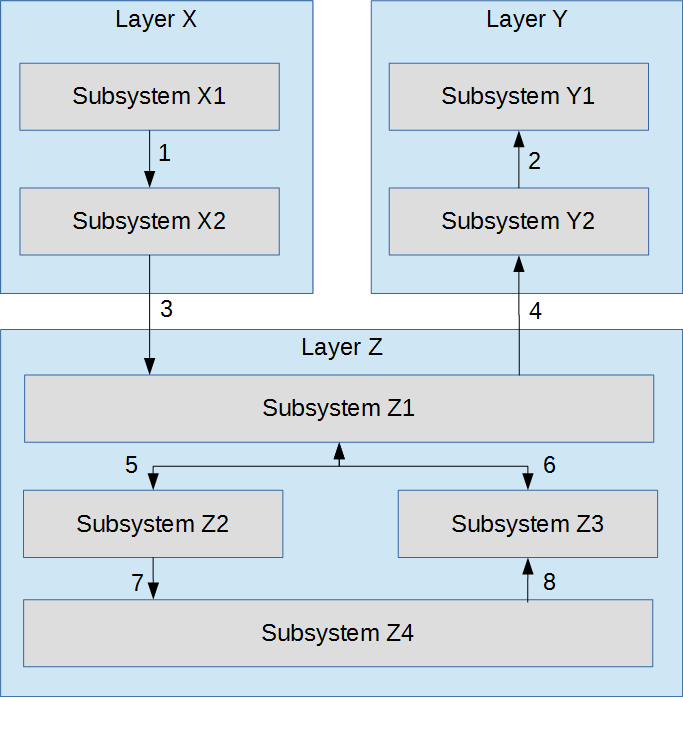
\includegraphics[width=0.90\textwidth]{images/data_flow}
 \caption{System architecture}
\end{figure}

\section{Roles \& Responsibilities}
The main stakeholder of our project is Frank Gronteman and CSE-4316 Professor Christopher D. McMurrough. Frank is an engineer and want to make the smart shutter project in a commercial level. The smart shutter will be developed to be used in commercial buildings like hospital, senior retirement homes and residential homes and business areas. \newline
Since the responsibility of the project has 3 separate teams which include EE team, embedded team and application team. EE team has the responsibility of developing the hardware and controller that controls the smart shutter. Embedded development team and our teams will work in microcontroller firmware, communication protocol and app interface. The project contains 3 teams; therefore, communication and exchange of information is a must. We would be communicating with teams and sponsors via an app called GroupMe. We have created the groups for all the teams and its members and sponsors to chat about the project. \newline
Since everyone is busy, we have decided to use GroupMe app and share their work through the app. Everyone will contribute in accomplishing the project. We can contact Frank via cellphone, email and GroupMe app. He has shared us his contact information in our recent meeting. Frank will hold the meetings in which we can discuss about our progress in the project. \newline
For our team, we will be chatting through GroupMe. We are going to meet with each other after the class for 15 minutes as sprint meeting and discuss about the project and assign the topic to be solved. We will have to divide the work and accomplish the task. If anyone cannot figure out the topic then we will bring that topic to everyone attention and try to solve it through meetings and discussion. If we need to have extra meeting, then we will fix the date and time through sprint meeting. \newline
Our application team members are as follows: 
Alejandro Escobar
Umesh Shrestha
Khoa Huynh
Tamunonengiye Nga
Jose Quintero

\section{Cost Proposal}
The major cost expenses will come from any libraries or software needed to complete the application. The software needed is dependent on the requirements of our application. The application will need to be on both Android and iOS devices. We will have one language and one implementation for both devices in order to reduce development time. The language will also depend on the protocols used in connecting with the Smart Shutters. It has not yet been decided how we are going to connect with them since the CSE team in charge of the firmware needs to decide with us if we want to connect the Smart Shutters to a central Hub via Bluetooth and then connect the Hub to our application via network/WiFi connection. 


\subsection{Preliminary Budget}
 Licenses - $200 \newline
Cloud storage - $200


\subsection{Current \& Pending Support}
Initial funding is provided to us by the University of Texas at Arlington. We begin with an 800 dollar budget. The sponsor, Frank Groenteman, is also providing funding but has not specified an exact dollar amount. Due to our project being mainly software based. 

\section{Facilities \& Equipment}
We have to work with two more difference teams for this project, one EE team and one more CSE team. This project required to create a circuit board with a chip that can receive a signal from an application to do action shut and open. We need electrical lap to create and testing the circuit board, that require soldering tool, electrical component for the board like resistor, capacitor, fuse, relay, transistor ... beside that we need and electric motor to create a force. A good design tool like Solidworks is needed for design circuit board. App team need computer with software to create android app and iOS app.\newline
Testing is needed all three teams to test separate first and collapse later for final test to make sure everything connect and working perfectly. We use electric testing kit like ohmmeter to check electric stuff and use unit testing to check our code.  For using the design and coding software we need to take time to look up and learn on google. There are some online class teaching how to code and design but we try to use both way to help us saving time to get our work done. All the electrical tools we use are available in the laps like pliers,magnetic screwdrivers.We do have 3D printer in the lap too but we have to pay for the material 1.75mm PLA Filament. There are some color for the filament with difference price and we chose the cheapest to save money. We also try to print our gear instead of order them form Amazon. \newline 
Some electrical components like chips, resistors, etc we need to order from Amazon or Ebay.\newline
Software are free to download and install and we just use our computer. We also use Github to share code, Slack and Groupme communicate with stakeholders and sponsors.We create two groups of Groupme, one for our team and one for sponsor communication. In that way we can keep track of our work and have more efficient way to communicate with team mate and sponsor.  





\section{Assumptions}

\begin{itemize}
  \item The EE team would complete a suitable prototype of the hardware portion of the project by the 3rd sprint.

  \item The CSE team working on the firmware would complete a suitable prototype of their portion of the project by the 4th sprint.

  \item The application prototype for the project would be finalized by the 4th sprint.

  \item A working prototype of the entire system would be accomplished by the 7th sprint

  \item After rigorous testing, the final product would be available for use by the 8th sprint

\end{itemize}
\section{Constraints}

\begin{itemize}
  \item The application development team is expected to work without a budget.

  \item The EE team working on the hardware has to have a viable product ready before the CSE team can test and configure the firmware.
  
  \item The CSE team working on the firmware has to have a reasonably complete setup of their portion of the product before the applications can be tested.

  \item The applications should be completed before the 7th sprint.

  \item A working product of the project is expected to be completed by the 8th sprint.

\end{itemize}

\section{Risks}
This section should contain a list of at least 5 of the most critical risks related to your project. Additionally, the probability of occurrence, size of loss, and risk exposure should be listed. For size of loss, express units as the number of days by which the project schedule would be delayed. For risk exposure, multiply the size of loss by the probability of occurrence to obtain the exposure in days. For example:

The following high-level risk census contains identified project risks with the highest exposure. Mitigation strategies will be discussed in future planning sessions.

\begin{table}[h]
\resizebox{\textwidth}{!}{
\begin{tabular}{|l|l|l|l|}
\hline
 \textbf{Risk description} & \textbf{Probability} & \textbf{Loss (days)} & \textbf{Exposure (days)} \\ \hline
 Availability of X sensor module due to contractor delay  & 0.50 & 20 & 10 \\ \hline
 Outdoor testing grounds are not available  & 0.20 & 14 & 2.8 \\ \hline
 Internet access not available at installation site  & 0.30 & 9 & 2.7 \\ \hline
 Delays in shipping from overseas vendors  & 0.10 & 20 & 2.0 \\ \hline
 Certification delays at compliance testing facility & 0.15 & 10 & 1.5 \\ \hline
\end{tabular}}
\caption{Overview of highest exposure project risks} 
\end{table}
\section{Documentation \& Reporting}
%%% In this section, you will describe all of the various artifacts that you will generate and maintain during the project life cycle. Describe the purpose of each item below, how the content will be generated, where it will be stored, how often it will be updated, etc. Replace the default text for each section with your own description. Reword this paragraph as appropriate.

\subsection{Major Documentation Deliverables}


\subsubsection{Project Charter}
The first draft of the project charter is due on October 1st, 2019. It will be maintained by all members of our project group and will maintained on OverLeaf. If new information is ever discovered or presented to us by another project team, the sponsor (Frank Groenteman), or our professor (Christopher McMurrough). Versions will be indicated at the beginning of the project charter. 

\subsubsection{System Requirements Specification}
The system requirements specification will be worked on during Sprint 2 (October 4th - October 21st). It will be maintained using a google spreadsheet shared among the project group members. Any additional requirements will be presented to us by another project team, the sponsor (Frank Groenteman), or our professor (Christopher McMurrough) and will be updated accordingly.


\subsubsection{Architectural Design Specification}
The architecture design specification will be worked on during Sprint 3 (October 25th - November 11th). 

\subsubsection{Detailed Design Specification}
The detailed design specification will be worked on during Sprint 2 (October 4th - October 21st).

\subsection{Recurring Sprint Items}

\subsubsection{Product Backlog}

After each meeting, if there is an item that should be added our team will start with voting. Because we work on application so most of the item will be use case and need com firm form sponsor.
\subsubsection{Sprint Planning}

Our sprint will be plan every 2 weeks so our team will have 4 meeting before sprint. 

\subsubsection{Sprint Goal}

Our team leader will decide our sprint goal. The process will be update with our sponsor by email or Groupme.
\subsubsection{Sprint Backlog}

Scrum master will decides  which product backlog items make their way into the sprint backlog. We will use Excel to maintain our Sprint Backlog.
\subsubsection{Task Breakdown}

Each tasks will be assigned to team mate base on which them prefer. Each team member will volunteer to claim task on meeting. Time spent will depend on the difficult of every tasks but no more than 2 weeks.

\subsubsection{Sprint Burn Down Charts}

Scrum master will responsible for generating the burn down charts for each sprint base on the product backlog and the time when team member submit task. The example of our burn down chart is showed below. We will have task and time. X-Axis is the project/iteration timeline, Y-Axi is the work that needs to be completed for the project. The time or story point estimates for the work remaining will be represented by this axis. Ideal Work Remaining Line is a straight line that connects the start point to the end point. Actual Work Remaining Line shows the actual work remaining.

\begin{figure}[h!]
    \centering
    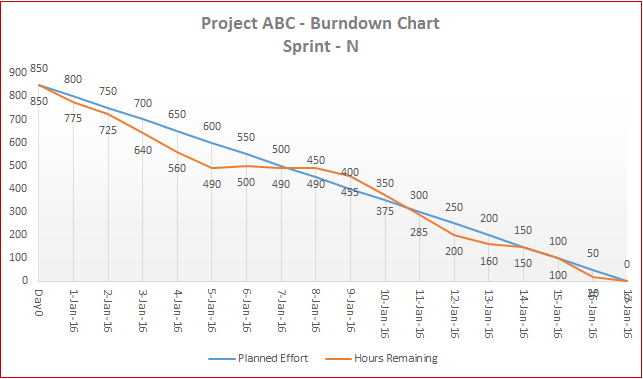
\includegraphics[width=0.5\textwidth]{images/burn_down_chart}
    \caption{Sprint burn down chart}
\end{figure}

\subsubsection{Sprint Retrospective}

The discussion will be on Monday after sprint, and sprint retrospective one of the subject of the meeting. The solution or help will be mention for each individual and the document will be done on Friday.


\subsubsection{Individual Status Reports}

The individual task will be report by each team member every sprint. We will use a share document online to report our process. It will show done or in process.
\subsubsection{Engineering Notebooks}
 
The minimum update of the the engineering notebook will be every meeting on Monday. Each interval will be 5-10 pages as needed, it will depend one how team member working and research about their task. Team will review work submit to keep each member accountable. Every team member except the owner can sign of "witness" for for each ENB page. 
\subsection{Closeout Materials}


\subsubsection{System Prototype}
In the final system prototype, all parts of this project will need to be working. The prototype will consist of the hardware (EE team), firmware (other CS team), and application team (our CS team). It will be due in May, 2020. It will be demonstrated by executing various tests to the Smart Shutters. These tests will be decided on at a later date by the sponsor, Frank Groenteman.


\subsubsection{Project Poster}
The project poster due date has not yet been specified by the instructor. Details will be added at a later date.

\subsubsection{Web Page}
The web page due date has not yet been specified by the instructor. Details will be added at a later date.


\subsubsection{Demo Video}
A demo video will be completed after the prototype is delivered. It will demo all the major functionalities of our application. It will contain video cuts showcasing each functionality. It will only be about 2-3 minutes long.

\subsubsection{Source Code}
Source code will be maintained by everyone in our project using Github. We have yet to discuss how the source code or executable will be presented to the other groups and/or the sponsor.

\subsubsection{Source Code Documentation}
Source documentation will be dependent on the programming language we use. For instance, if you Java is used, we will be generating a Javadoc.






\subsubsection{Installation Scripts}
Installation scripts have not yet been decided. This will be populated once the system requirements, architecture, and design specifications have been completed.

\subsubsection{User Manual}
A digital user manual will be created upon request from the sponsor, Frank Groenteman. Alternatively, the demo video can be provided as the user’s manual.


\newpage

%%% References
\bibliographystyle{plain}
\bibliographystyle{reference/IEEEtran_custom}
\bibliography{reference/library}{}

\end{document}